\section{时变系统}
\label{sec:lde-time-varying}

系数矩阵随时间变化时，方程变成
\begin{equation}
 \dot{\bm{x}}(t)=\bm{A}(t)\bm{x}(t),\qquad \bm{x}(s)=\bm{\xi},
 \label{eq:lde-time-varying}
\end{equation}
其中$\bm{A}:I\to\mathbb{R}^{n\times n}$在区间$I$上连续，$s\in I$。一个自然的想法是照搬标量公式，用$\exp\int_s^t\bm{A}$作传播。这个想法一般是错的，错在哪里要等传播矩阵本身建立好才能说清。所以先回答：不写闭式，能否定义出从时刻$s$到时刻$t$的线性传播？

\paragraph{用迭代造出传播矩阵}
把方程~\eqref{eq:lde-time-varying}对时间积分，得到
\[
 \bm{x}(t)=\bm{\xi}+\int_s^t\bm{A}(r)\bm{x}(r)\,\mathrm{d}r.
\]
解出现在右端，于是把右端的$\bm{x}$反复用整个等式代入。第一次代入后多出一项，第二次代入后再多一项，一直做下去，得到矩阵的级数
\begin{equation}
 \begin{aligned}
 \bm{\Phi}(t,s)={}&\bm{I}+\int_s^t\bm{A}(r_1)\,\mathrm{d}r_1\\
 &+\int_s^t\!\!\int_s^{r_1}\bm{A}(r_1)\bm{A}(r_2)\,\mathrm{d}r_2\,\mathrm{d}r_1+\cdots,
 \end{aligned}
 \label{eq:lde-peano-baker}
\end{equation}
称为\term{Peano--Baker级数}（Peano--Baker series）。第$k$项是$k$重积分，被积函数中时间较晚的因子写在左边。

这个级数是矩阵指数的时间排序版本。$\bm{A}$是常数时，第$k$项被积函数恒为$\bm{A}^k$，积分区域$s\leq r_k\leq\cdots\leq r_1\leq t$的体积是$(t-s)^k/k!$，第$k$项就是$(t-s)^k\bm{A}^k/k!$，级数回到式~\eqref{eq:lde-matrix-exponential}。阶乘的来历也清楚了：它是$k$个时刻按先后排列的区域在立方体中所占的比例。

\begin{definition}[状态转移矩阵]
\label{def:lde-transition}
设$\bm{A}$在$I$上连续，$s\in I$。把矩阵初值问题
\begin{equation}
 \partial_t\bm{\Phi}(t,s)=\bm{A}(t)\bm{\Phi}(t,s),\qquad \bm{\Phi}(s,s)=\bm{I}
 \label{eq:lde-transition}
\end{equation}
的解称为\term{状态转移矩阵}（state transition matrix）。第一个自变量$t$是终止时刻，第二个自变量$s$是初始时刻。
\end{definition}

\begin{theorem}[线性系统的整体存在唯一]
\label{thm:lde-transition-existence}
设$\bm{A}$在$I$上连续。对每个$s\in I$，问题~\eqref{eq:lde-transition}在整个$I$上有唯一解，由级数~\eqref{eq:lde-peano-baker}给出。对每个$\bm{\xi}\in\mathbb{R}^n$，方程~\eqref{eq:lde-time-varying}在$I$上的唯一解是
\begin{equation}
 \bm{x}(t)=\bm{\Phi}(t,s)\bm{\xi}.
 \label{eq:lde-transition-solution}
\end{equation}
\end{theorem}

\begin{proof}
取含$s$的紧子区间$J\subset I$，定义累积系数大小
\[
 \alpha(t)=\Bigl\lvert\int_s^t\lVert\bm{A}(r)\rVert_2\,\mathrm{d}r\Bigr\rvert.
\]
记级数第$k$项为$\bm{T}_k(t)$，它满足$\bm{T}_0=\bm{I}$和递推关系
\[
 \bm{T}_{k+1}(t)=\int_s^t\bm{A}(r)\bm{T}_k(r)\,\mathrm{d}r.
\]
归纳可得$\lVert\bm{T}_k(t)\rVert_2\leq\alpha(t)^k/k!$，归纳一步是
\[
 \lVert\bm{T}_{k+1}(t)\rVert_2\leq\Bigl\lvert\int_s^t\lVert\bm{A}(r)\rVert_2\frac{\alpha(r)^k}{k!}\,\mathrm{d}r\Bigr\rvert=\frac{\alpha(t)^{k+1}}{(k+1)!}.
\]

$\alpha$在$J$上有界，由优级数判别法，级数在$J$上一致收敛到连续的矩阵函数$\bm{\Phi}(\cdot,s)$。把递推式对$k$求和，并在一致收敛下交换求和与积分，得到
\[
 \bm{\Phi}(t,s)=\bm{I}+\int_s^t\bm{A}(r)\bm{\Phi}(r,s)\,\mathrm{d}r.
\]
被积函数连续，所以$\bm{\Phi}$对$t$连续可微，满足式~\eqref{eq:lde-transition}。$J$可以任取，所以解在整个$I$上存在。

再证唯一。设向量函数$\bm{y}$满足$\dot{\bm{y}}=\bm{A}\bm{y}$、$\bm{y}(s)=\bm{0}$，令$B=\max_J\lVert\bm{y}\rVert_2$。积分形式给出$\lVert\bm{y}(t)\rVert_2\leq B\alpha(t)$，代回积分形式再估计，反复进行，得到对每个$k$都有
\[
 \lVert\bm{y}(t)\rVert_2\leq\frac{B\alpha(t)^k}{k!}.
\]
令$k\to\infty$得$\bm{y}\equiv\bm{0}$。把它用于两个解之差，矩阵方程按列处理，就得到两个问题解的唯一性。式~\eqref{eq:lde-transition-solution}满足方程~\eqref{eq:lde-time-varying}可以直接代入验证。
\end{proof}

第~\ref{chap:ode-existence-continuation}章会把同样的迭代用于非线性方程，那里一般只能得到局部结论。线性方程的估计不受状态大小的影响，所以结论对整个$I$成立。若$\bm{A}$只是分段连续，就在每一段上求解，并在接缝处把状态接起来，$\bm{\Phi}$仍然连续，只是对$t$的导数在接缝处有跳变。

\paragraph{基本解矩阵}
实际求解时，往往是先设法找到$n$个线性无关的解，再组装成传播矩阵。

\begin{definition}[基本解矩阵]
\label{def:lde-fundamental-matrix}
若矩阵函数$\bm{X}:I\to\mathbb{R}^{n\times n}$连续可微，满足下式，并且在某一时刻可逆，就称它为\term{基本解矩阵}（fundamental matrix）：
\begin{equation}
 \dot{\bm{X}}(t)=\bm{A}(t)\bm{X}(t).
 \label{eq:lde-fundamental-matrix}
\end{equation}
\end{definition}

它的$n$列是$n$个解。若$\bm{X}$在某时刻$t_*$可逆，则它在每个时刻都可逆。否则存在时刻$t_1$和$\bm{c}\neq\bm{0}$使$\bm{X}(t_1)\bm{c}=\bm{0}$；而$\bm{X}(t)\bm{c}$是解，在$t_1$为零，由唯一性恒为零，这与$\bm{X}(t_*)$可逆矛盾。

由定义~\ref{def:lde-transition}的唯一性，$\bm{X}(t)\bm{X}(s)^{-1}$就是$\bm{\Phi}(t,s)$，因为它对$t$满足同一方程，在$t=s$时等于$\bm{I}$：
\begin{equation}
 \bm{\Phi}(t,s)=\bm{X}(t)\bm{X}(s)^{-1}.
 \label{eq:lde-fundamental-to-transition}
\end{equation}

这个公式可以理解为换坐标。$\bm{X}(s)^{-1}$把时刻$s$的状态写成$n$个基本解在该时刻取值的组合，得到组合系数。方程是线性的，组合系数不随时间改变。再用时刻$t$的基本解按同样的系数组合，就读出了时刻$t$的状态。

\begin{theorem}[状态转移矩阵的性质]
\label{thm:lde-transition-properties}
对$r,s,t\in I$，下列性质成立，时刻的大小次序不限。
\begin{enumerate}
 \item 复合：
 \begin{equation}
  \bm{\Phi}(t,r)\bm{\Phi}(r,s)=\bm{\Phi}(t,s).
  \label{eq:lde-transition-composition}
 \end{equation}
 \item 可逆：$\bm{\Phi}(t,s)$可逆，并且
 \begin{equation}
  \bm{\Phi}(t,s)^{-1}=\bm{\Phi}(s,t).
  \label{eq:lde-transition-inverse}
 \end{equation}
 \item 对初始时刻求导：
 \begin{equation}
  \partial_s\bm{\Phi}(t,s)=-\bm{\Phi}(t,s)\bm{A}(s).
  \label{eq:lde-transition-initial-derivative}
 \end{equation}
 \item 常系数情形：若$\bm{A}(t)\equiv\bm{A}$，则$\bm{\Phi}$只依赖$t-s$：
 \begin{equation}
  \bm{\Phi}(t,s)=\mathrm{e}^{(t-s)\bm{A}}.
  \label{eq:lde-transition-constant}
 \end{equation}
\end{enumerate}
\end{theorem}

\begin{proof}
取$\bm{X}(t)=\bm{\Phi}(t,t_*)$作为基本解矩阵，其中$t_*\in I$任意。代入式~\eqref{eq:lde-fundamental-to-transition}，(1)就是
\[
 \bm{X}(t)\bm{X}(r)^{-1}\bm{X}(r)\bm{X}(s)^{-1}=\bm{X}(t)\bm{X}(s)^{-1}.
\]
(2)由$\bm{X}(s)\bm{X}(t)^{-1}$是$\bm{X}(t)\bm{X}(s)^{-1}$的逆得到。

(3)对$\bm{X}(s)^{-1}\bm{X}(s)=\bm{I}$求导，得到恒等式
\[
 \partial_s\bigl(\bm{X}(s)^{-1}\bigr)=-\bm{X}(s)^{-1}\dot{\bm{X}}(s)\bm{X}(s)^{-1}.
\]
代入$\dot{\bm{X}}=\bm{A}\bm{X}$，并左乘$\bm{X}(t)$，得
\[
 \partial_s\bm{\Phi}(t,s)=-\bm{X}(t)\bm{X}(s)^{-1}\bm{A}(s)=-\bm{\Phi}(t,s)\bm{A}(s).
\]

(4)由定理~\ref{thm:lde-constant-solution}，$\mathrm{e}^{(t-s)\bm{A}}$满足式~\eqref{eq:lde-transition}，由唯一性得结论。
\end{proof}

两个时刻的角色并不对称。对终止时刻求导，系数矩阵$\bm{A}(t)$乘在左边，表示最后这一小段的传播作用在最外层。对初始时刻求导，$-\bm{A}(s)$乘在右边，表示最开始的那一小段被去掉。图~\ref{fig:lde-transition-composition}是复合关系的示意：先从$s$传到$r$，再从$r$传到$t$，与直接从$s$传到$t$结果相同。

\begin{BookInlineFigure}
  \centering
  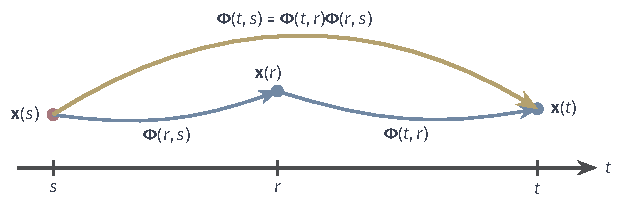
\includegraphics[width=105mm]{figures/06-differential-equations/01-ordinary-differential-equations/tikz/lde-transition-composition/figure.pdf}
  \caption{状态转移矩阵的复合。横轴是时间，红点是时刻$s$的状态，蓝点是其后的状态。两段蓝色箭头依次传播，黄色箭头直接传播，二者结果相同。矩阵乘积中晚的时刻写在左边。}
  \label{fig:lde-transition-composition}
\end{BookInlineFigure}

\begin{example}[一个可解的时变系统]
\label{ex:lde-time-varying}
取
\[
 \bm{A}(t)=\begin{bmatrix}0&t\\0&1\end{bmatrix},
\]
方程是$\dot{x}_1=tx_2$、$\dot{x}_2=x_2$。第二个方程先解出$x_2=\mathrm{e}^{t}x_2(0)$。代入第一个方程，再用分部积分，可知$t\mathrm{e}^{t}$的一个原函数是$(t-1)\mathrm{e}^{t}$。

于是$(1,0)^{\top}$和$((t-1)\mathrm{e}^{t},\mathrm{e}^{t})^{\top}$是两个解，把它们并排放置，得到基本解矩阵和它的逆：
\[
 \bm{X}(t)=\begin{bmatrix}1&(t-1)\mathrm{e}^{t}\\0&\mathrm{e}^{t}\end{bmatrix},\qquad
 \bm{X}(s)^{-1}=\begin{bmatrix}1&1-s\\0&\mathrm{e}^{-s}\end{bmatrix}.
\]
由式~\eqref{eq:lde-fundamental-to-transition}，
\[
 \bm{\Phi}(t,s)=\begin{bmatrix}1&(1-s)+(t-1)\mathrm{e}^{t-s}\\0&\mathrm{e}^{t-s}\end{bmatrix}.
\]
取$t=s$，右上角为$(1-s)+(s-1)=0$，符合$\bm{\Phi}(s,s)=\bm{I}$。再取时长都是$1$的两段：
\[
 \bm{\Phi}(1,0)=\begin{bmatrix}1&1\\0&\mathrm{e}\end{bmatrix},\qquad
 \bm{\Phi}(2,1)=\begin{bmatrix}1&\mathrm{e}\\0&\mathrm{e}\end{bmatrix}.
\]
它们不相等，说明传播同时依赖两个时刻，而不只依赖时长。它们的乘积是
\[
 \bm{\Phi}(2,1)\bm{\Phi}(1,0)=\begin{bmatrix}1&1+\mathrm{e}^2\\0&\mathrm{e}^2\end{bmatrix},
\]
这正是公式给出的$\bm{\Phi}(2,0)$，复合关系得到验证。
\end{example}

\paragraph{为什么不能积分后取指数}
现在可以检验开始时的想法了。对例~\ref{ex:lde-time-varying}的系数，从$0$积分得到
\[
 \bm{M}(t)=\int_0^t\bm{A}(r)\,\mathrm{d}r=\begin{bmatrix}0&t^2/2\\0&t\end{bmatrix}.
\]
固定$t$，写$\bm{M}=t\bm{B}$，其中$\bm{B}$满足$\bm{B}^2=\bm{B}$：
\[
 \bm{B}=\begin{bmatrix}0&t/2\\0&1\end{bmatrix}.
\]
于是级数中$\bm{B}^k$全部等于$\bm{B}$，求和得到
\[
 \mathrm{e}^{\bm{M}(t)}=\bm{I}+(\mathrm{e}^{t}-1)\bm{B}=\begin{bmatrix}1&(\mathrm{e}^{t}-1)t/2\\0&\mathrm{e}^{t}\end{bmatrix}.
\]

把它与$\bm{\Phi}(t,0)$的右上角比较：真解是$(t-1)\mathrm{e}^{t}+1$，直接取指数的结果是$(\mathrm{e}^{t}-1)t/2$。取$t=2$，前者是$\mathrm{e}^2+1\approx8.389$，后者是$\mathrm{e}^2-1\approx6.389$。图~\ref{fig:lde-noncommuting}中两条曲线随时间逐渐分开，绿点是对原方程作数值积分的结果，它落在蓝线上。

\begin{BookInlineFigure}
  \centering
  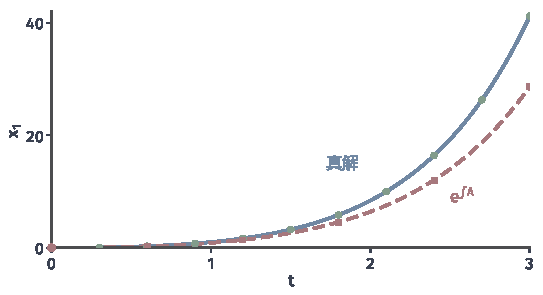
\includegraphics[width=92mm]{figures/06-differential-equations/01-ordinary-differential-equations/matplotlib/lde-noncommuting/figure.pdf}
  \caption{时变系统不能对系数积分后直接取指数。$\bm{A}(t)=\left[\begin{smallmatrix}0&t\\0&1\end{smallmatrix}\right]$，$\bm{x}(0)=(0,1)^{\top}$，图中是分量$x_1$。蓝线是真解$(t-1)\mathrm{e}^{t}+1$，绿点是步长$0.05$的四阶Runge--Kutta数值解；红色虚线是$\exp\int_0^t\bm{A}$给出的$(\mathrm{e}^{t}-1)t/2$，红色方点是对$\bm{M}(t)$直接计算矩阵指数的结果。}
  \label{fig:lde-noncommuting}
\end{BookInlineFigure}

失败的原因在求导。若想让$\mathrm{e}^{\bm{M}(t)}$满足方程，$\mathrm{e}^{\bm{M}}$的导数就要等于$\dot{\bm{M}}\mathrm{e}^{\bm{M}}$。看级数中的二次项：
\[
 \frac{\mathrm{d}}{\mathrm{d}t}\bm{M}^2=\dot{\bm{M}}\bm{M}+\bm{M}\dot{\bm{M}}.
\]
只有$\dot{\bm{M}}$与$\bm{M}$可交换时，它才等于$2\dot{\bm{M}}\bm{M}$。例中$\bm{A}(s)\bm{A}(t)=\bm{A}(s)$而$\bm{A}(t)\bm{A}(s)=\bm{A}(t)$，两个时刻的系数不可交换。

从传播的角度看更直观。$\exp\int\bm{A}$把各时刻的系数不分先后地加在一起，Peano--Baker级数却严格保留“晚的在左”的次序。图~\ref{fig:lde-switching-order}用两段常系数的切换说明次序的影响。设两段系数各作用单位时间：
\[
 \bm{A}_1=\begin{bmatrix}0&1\\0&0\end{bmatrix},\qquad \bm{A}_2=\begin{bmatrix}0&0\\1&0\end{bmatrix}.
\]
由$\bm{A}_1^2=\bm{A}_2^2=\bm{0}$，得$\mathrm{e}^{\bm{A}_i}=\bm{I}+\bm{A}_i$。

先用$\bm{A}_1$、后用$\bm{A}_2$的传播是
\[
 \mathrm{e}^{\bm{A}_2}\mathrm{e}^{\bm{A}_1}=\begin{bmatrix}1&1\\1&2\end{bmatrix}.
\]
次序反过来的传播是
\[
 \mathrm{e}^{\bm{A}_1}\mathrm{e}^{\bm{A}_2}=\begin{bmatrix}2&1\\1&1\end{bmatrix}.
\]
两种切换的系数积分都是$\bm{A}_1+\bm{A}_2$，而直接取指数得到
\[
 \mathrm{e}^{\bm{A}_1+\bm{A}_2}=\begin{bmatrix}\cosh1&\sinh1\\\sinh1&\cosh1\end{bmatrix},
\]
与两者都不同。这就像先向右剪切再向上剪切，与先向上剪切再向右剪切，结果是两个不同的平行四边形。

\begin{BookInlineFigure}
  \centering
  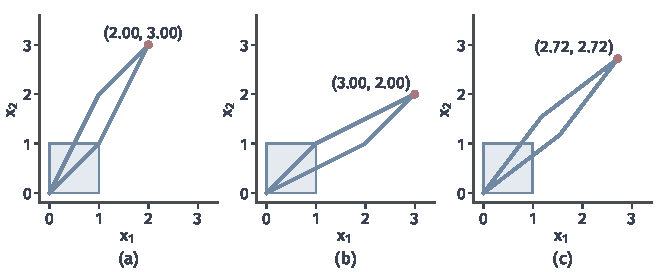
\includegraphics[width=112mm]{figures/06-differential-equations/01-ordinary-differential-equations/matplotlib/lde-switching-order/figure.pdf}
  \caption{切换次序影响结果，浅蓝方块是单位正方形，蓝线是它的像，红点是$(1,1)^{\top}$的像。(a)$\mathrm{e}^{\bm{A}_2}\mathrm{e}^{\bm{A}_1}$。(b)$\mathrm{e}^{\bm{A}_1}\mathrm{e}^{\bm{A}_2}$。(c)$\mathrm{e}^{\bm{A}_1+\bm{A}_2}$，它对应系数积分后直接取指数，不等于任何一种切换次序的实际传播。}
  \label{fig:lde-switching-order}
\end{BookInlineFigure}

\paragraph{可交换时的简化}
上面的分析也指出了简化公式成立的条件：让所有时刻的系数彼此可交换。

\begin{theorem}[可交换系数的状态转移矩阵]
\label{thm:lde-commuting}
设$\bm{A}$在$I$上连续，并且对任意$r,r'\in I$都有$\bm{A}(r)\bm{A}(r')=\bm{A}(r')\bm{A}(r)$。则
\begin{equation}
 \bm{\Phi}(t,s)=\exp\Bigl(\int_s^t\bm{A}(r)\,\mathrm{d}r\Bigr).
 \label{eq:lde-commuting}
\end{equation}
\end{theorem}

\begin{proof}
固定$s$，令$\bm{M}(t)=\int_s^t\bm{A}(r)\,\mathrm{d}r$。积分是Riemann和的极限，而每个Riemann和都与$\bm{A}(t)$可交换，所以$\bm{M}(t)\bm{A}(t)=\bm{A}(t)\bm{M}(t)$。

用乘积求导并归纳，$\frac{\mathrm{d}}{\mathrm{d}t}\bm{M}^k$是$k$项之和，每一项都把一个因子$\bm{M}$换成$\bm{A}(t)$。交换关系把$\bm{A}(t)$移到最左边，得到
\[
 \frac{\mathrm{d}}{\mathrm{d}t}\bm{M}^k=k\bm{A}(t)\bm{M}^{k-1}.
\]
逐项求导的级数在紧子区间上被$\lVert\bm{A}(t)\rVert_2\mathrm{e}^{\lVert\bm{M}(t)\rVert_2}$的同型优级数控制，所以求导合法，并且
\[
 \frac{\mathrm{d}}{\mathrm{d}t}\mathrm{e}^{\bm{M}(t)}=\bm{A}(t)\mathrm{e}^{\bm{M}(t)}.
\]
又有$\bm{M}(s)=\bm{0}$，由定理~\ref{thm:lde-transition-existence}的唯一性得到结论。
\end{proof}

定理的条件是充分条件。标量方程、对角系数和$\bm{A}(t)=a(t)\bm{B}$（$\bm{B}$为常矩阵）都满足它。最后一种情形有直观的含义：$a(t)$只决定沿$\bm{B}$的轨线走得多快，不改变轨线本身。例如$\bm{A}(t)=2t\bm{J}_0$时，式~\eqref{eq:lde-commuting}给出
\[
 \bm{\Phi}(t,0)=\mathrm{e}^{t^2\bm{J}_0}=\begin{bmatrix}\cos t^2&\sin t^2\\-\sin t^2&\cos t^2\end{bmatrix}.
\]
状态仍在圆周上转动，只是把时间换成了$t^2$。一般的时变系统没有这种闭式，$\bm{\Phi}$要靠数值方法求解，这由第~\ref{chap:ode-numerical-methods}章讨论。
